\documentclass[11pt,a4paper]{article}

\usepackage[utf8]{inputenc}
\usepackage[T1]{fontenc}
\usepackage[spanish]{babel}
\usepackage{geometry}
\usepackage{graphicx}
\usepackage{array}
\usepackage{tabularx}
\usepackage{makecell}
\usepackage[table]{xcolor}
\usepackage{fancyhdr}
\usepackage{titlesec}
\usepackage{helvet}
\usepackage{ragged2e}
\usepackage{enumitem}
\usepackage{setspace}
\usepackage{hyperref}
\usepackage{booktabs} % Para tablas con acabado profesional
\usepackage{alltt}    % Bloque monoespaciado que si admite macros (lambda, mu, rho)
\usepackage{amsmath}  % Para las formulas del modelo

\renewcommand{\familydefault}{\sfdefault}
\geometry{
  a4paper,
  left=3.0cm,
  right=3.0cm,
  top=2.35cm,
  bottom=2.35cm,
  headheight=1.9cm,
  headsep=0.45cm
}

\setlength{\parindent}{0pt}
\setlength{\parskip}{0.22em}
\setlength{\emergencystretch}{2em}   % evita desbordes de linea en texto justificado
\setlength{\tabcolsep}{6pt}
\renewcommand{\arraystretch}{1.08}

\pagestyle{fancy}
\fancyhf{}
\fancyhead[L]{
\includegraphics[height=1.35cm]{assets/reporte_tecnico_overleaf_logo.png}}
\fancyhead[R]{\vspace{0.1cm}\small FEIRNNR - Carrera de Computación}
\renewcommand{\headrulewidth}{0.5pt}
\renewcommand{\footrulewidth}{0pt}
\makeatletter
\renewcommand{\headrule}{%
  {\color{gray!65}\hrule width\headwidth height\headrulewidth \vskip-\headrulewidth}%
}
\makeatother

\titleformat{\section}
  {\bfseries\fontsize{15}{17}\selectfont}
  {\thesection.}{0.8em}{}
\titlespacing*{\section}{0pt}{0.7ex}{0.2ex}

\newcolumntype{L}[1]{>{\RaggedRight\arraybackslash}p{#1}}
\newcolumntype{Y}{>{\RaggedRight\arraybackslash}X}

% Marca visible de lo que el equipo todavia debe escribir.
\newcommand{\pendiente}[1]{\textcolor{red}{\textbf{[PENDIENTE: #1]}}}

% Paleta de las tablas de la plantilla institucional.
\definecolor{headerblue}{RGB}{19, 93, 126}
\definecolor{rowlight}{RGB}{205, 235, 248}
\definecolor{borderblue}{RGB}{64, 160, 206}

% babel-espanol renombra \tablename como "Cuadro"; el texto usa "Tabla".
\addto\captionsspanish{\renewcommand{\tablename}{Tabla}}

\begin{document}
\thispagestyle{fancy}

\vspace*{0.15cm}

\begin{center}
{\bfseries\fontsize{23}{26}\selectfont
Reporte Técnico de Actividades\\
Práctico-Experimentales Nro. 003\par}
\end{center}

\section{Datos de Identificación del Estudiante y la Práctica}

\noindent
\begin{tabularx}{\textwidth}{|L{0.43\textwidth}|Y|}
\hline
\textbf{Nombre del estudiante(s)} & Jaime Landázuri, Richard Chamba, Cael Soto, Domenica Rojas \\ \hline
\textbf{Asignatura} & Simulación \\ \hline
\textbf{Ciclo} & 5 A \\ \hline
\textbf{Unidad} & 1 \\ \hline
\textbf{Resultado de aprendizaje de la unidad} & R1. Aplica análisis estadísticos de los datos
de la Simulación para mejorar la calidad de los resultados, bajo los principios de solidaridad, transparencia, responsabilidad y honestidad. \\ \hline
\textbf{Práctica Nro.} & 003 \\ \hline
\textbf{Título de la Práctica} & Simulación de un sistema de líneas de espera M/M/1 mediante SimPy \\ \hline
\textbf{Nombre del Docente} & José O. Guamán Q. \\ \hline
\textbf{Fecha} & 15 de Octubre de 2026 \\
 & 16 de Octubre 2026 \\ \hline
\textbf{Horario} & Jueves 10h30 a 11h30 \\
 & Viernes 07h30 a 09h30 \\ \hline
\textbf{Lugar} & Aula \\ \hline
\textbf{Tiempo planificado en el Sílabo} & 3 horas \\ \hline
\end{tabularx}

\section{Objetivo(s) de la Práctica}
Simular un sistema de líneas de espera M/M/1 utilizando Python y SimPy, analizando
el comportamiento de los clientes, la cola y el servidor.
\begin{enumerate}
    \item Implementar un modelo M/M/1 utilizando la biblioteca SimPy.
    \item Calcular las principales métricas teóricas del sistema de espera.
    \item Comparar los resultados teóricos con los obtenidos mediante la simulación.
\end{enumerate}

\section{Materiales y reactivos}
\begin{itemize}
    \item Python 3.x (se ejecutó con Python 3.14.8).
    \item Biblioteca SimPy (se ejecutó con SimPy 4.1.2).
    \item NumPy (2.5.4).
    \item Matplotlib (3.11.2).
    \item Editor de código: Visual Studio Code, PyCharm o Jupyter Notebook.
\end{itemize}

\section{Equipos y herramientas}
\begin{itemize}
    \item Computador.
    \item Procesador de 2 núcleos o superior.
    \item Mínimo 4 GB de RAM.
    \item Sistema operativo Linux o macOS.
\end{itemize}

\section{Procedimiento / Metodología Ejecutada}

\subsection{Fundamento teórico}

El modelo \textbf{M/M/1} representa un sistema de líneas de espera con llegadas de
clientes siguiendo una distribución de Poisson, tiempos de servicio con distribución
exponencial, un único servidor y atención de clientes bajo el principio FIFO
(\emph{primero en llegar, primero en ser atendido}).

El modelo utiliza dos parámetros principales:
\begin{itemize}
    \item $\lambda$: tasa promedio de llegada de clientes.
    \item $\mu$: tasa promedio de servicio del servidor.
\end{itemize}

La utilización del servidor se calcula mediante:
\[
\rho = \frac{\lambda}{\mu}
\]

\noindent\textbf{Observación sobre la guía.} La guía de la práctica (§5.1) imprime
$\rho = \mu/\lambda$, lo que contradice su propia condición de estabilidad
$\lambda < \mu$ enunciada unas líneas más abajo y también su pseudocódigo, que usa
$\rho = \lambda/\mu$. Con la fórmula impresa, los tres escenarios de la guía darían
$\rho = 1{,}50$, $1{,}20$ y $1{,}03$, es decir un servidor saturado en los tres casos, y
las medidas $L$, $L_q$, $W$ y $W_q$ no existirían, porque solo están definidas para
$\rho < 1$. Este trabajo usa la definición correcta $\rho = \lambda/\mu$, que es la que
emplea el pseudocódigo de la propia guía y la que aparece en la bibliografía de teoría
de colas.

Para que el sistema sea estable debe cumplirse:
\[
\lambda < \mu
\]

Las principales medidas teóricas del sistema son:

\[
L = \frac{\lambda}{\mu-\lambda} \qquad
L_q = \frac{\lambda^2}{\mu(\mu-\lambda)}
\]

\[
W = \frac{1}{\mu-\lambda} \qquad
W_q = \frac{\lambda}{\mu(\mu-\lambda)}
\]

\begin{table}[h!]
\centering
\setlength{\arrayrulewidth}{0.75pt}
\arrayrulecolor{borderblue}
\renewcommand{\arraystretch}{1.25}
\begin{tabular}{|l|l|}
\hline
\rowcolor{headerblue}
\textbf{\textcolor{white}{Símbolo}} & \textbf{\textcolor{white}{Significado}} \\ \hline
$\lambda$ & Tasa de llegada de clientes \\ \hline
\rowcolor{rowlight}
$\mu$ & Tasa de servicio \\ \hline
$\rho$ & Utilización del servidor \\ \hline
\rowcolor{rowlight}
$L$ & Número promedio de clientes en el sistema \\ \hline
$L_q$ & Número promedio de clientes en la cola \\ \hline
\rowcolor{rowlight}
$W$ & Tiempo promedio en el sistema \\ \hline
$W_q$ & Tiempo promedio de espera en la cola \\ \hline
\end{tabular}
\caption{Notación empleada.}
\end{table}

\subsection{Escenarios ejecutados}

Se ejecutaron los tres escenarios indicados por la guía, todos con $\mu = 3{,}0$:

\begin{table}[h!]
\centering
\setlength{\arrayrulewidth}{0.75pt}
\arrayrulecolor{borderblue}
\renewcommand{\arraystretch}{1.25}
\begin{tabular}{|c|c|c|l|}
\hline
\rowcolor{headerblue}
\textbf{\textcolor{white}{Escenario}} & \textbf{\textcolor{white}{$\lambda$}} & \textbf{\textcolor{white}{$\mu$}} & \textbf{\textcolor{white}{Condición}} \\ \hline
1 & 2{,}0 & 3{,}0 & Sistema estable \\ \hline
\rowcolor{rowlight}
2 & 2{,}5 & 3{,}0 & Mayor utilización \\ \hline
3 & 2{,}9 & 3{,}0 & Cerca de saturación \\ \hline
\end{tabular}
\caption{Escenarios de la guía. La utilización teórica resulta $\rho = 0{,}667$,
$0{,}833$ y $0{,}967$ respectivamente.}
\end{table}

\subsection{Arquitectura e implementación}

El programa se desarrolló en Python siguiendo el pseudocódigo de la guía y se
estructuró en tres capas (modelo, vista y controlador) para que cada medida tuviera un
único responsable en el código. Los componentes son:

\begin{itemize}
    \item \textbf{Escenarios} (\path{modelo/escenarios.py}): cada escenario es un
    objeto con su $\lambda$, su $\mu$ y su condición. Para cambiar un escenario se
    editan sus números y para agregar uno nuevo se añade a la lista \texttt{ESCENARIOS}.
    \item \textbf{Métricas teóricas} (\path{modelo/teoria.py}): calcula $\rho$, $L$,
    $L_q$, $W$ y $W_q$ con las fórmulas del apartado anterior y expone
    \texttt{es\_estable()} para verificar $\lambda < \mu$. Actúa como \emph{oráculo} de
    correctitud del simulador.
    \item \textbf{Motor de simulación} (\path{modelo/simulacion.py}): crea un entorno
    SimPy con un servidor de \texttt{capacity = 1} y genera los clientes con tiempos
    entre llegadas exponenciales de tasa $\lambda$ (\texttt{expovariate}). Cada cliente
    pide el servidor, espera su turno en orden FIFO y es atendido con un tiempo
    exponencial de tasa $\mu$. Por cada cliente se registra el tiempo de espera en cola,
    y aparte se guarda una traza del tamaño de la cola a lo largo del tiempo.
    \item \textbf{Tablas} (\path{vista/tabla.py}): imprime en la terminal la tabla de
    valores teóricos y la tabla de teoría contra simulación. No calcula nada.
    \item \textbf{Gráficas} (\path{vista/graficas.py}): genera las tres figuras del
    informe y las guarda en \texttt{graficas/}.
    \item \textbf{Controlador} (\path{controlador/controlador.py}): recorre los
    escenarios, simula cada uno varias veces, promedia las réplicas y une el modelo con
    la vista. Si un escenario no cumple $\lambda < \mu$, avisa que el sistema no es
    estable, no lo simula y continúa con el siguiente.
    \item \textbf{Punto de entrada} (\path{main.py}): un solo comando ejecuta todo el
    estudio:
\end{itemize}

\begin{verbatim}
python3 main.py
\end{verbatim}

\noindent\textbf{Medición de las métricas simuladas.} Dos detalles de implementación
importan para que los números sean comparables con la teoría:

\begin{itemize}
    \item La \textbf{espera promedio} se calcula como el promedio simple de los tiempos
    de espera de todos los clientes atendidos en la corrida, que es un estimador de
    $W_q$ insesgado y de varianza decreciente con el número de clientes.
    \item El \textbf{tamaño promedio de la cola} no se calcula como el promedio de las
    muestras instantáneas, porque muestrear por evento sesgaría el resultado a favor de
    las colas cortas (que son las que más tiempo duran con pocos clientes). Se calcula
    como el \emph{promedio ponderado por tiempo}: cada tamaño de cola se multiplica por
    el tiempo que permaneció en ese valor y al final se divide entre el tiempo total
    simulado. Ese es el estimador correcto de $L_q$.
\end{itemize}

\noindent\textbf{Guarda de estabilidad.} Si en algún escenario $\lambda \geq \mu$ el
programa no simula: informa que el sistema no es estable y sigue con los demás. Esto
respeta el pseudocódigo de la guía y evita reportar promedios de una cola que crece sin
límite.

\subsection{Parámetros de la corrida oficial y reproducibilidad}

La corrida que alimenta este informe se ejecutó con la configuración definida en el
controlador, en el archivo \path{controlador/controlador.py}:

\begin{table}[h!]
\centering
\setlength{\arrayrulewidth}{0.75pt}
\arrayrulecolor{borderblue}
\renewcommand{\arraystretch}{1.25}
\begin{tabular}{|l|c|l|}
\hline
\rowcolor{headerblue}
\textbf{\textcolor{white}{Variable}} & \textbf{\textcolor{white}{Valor}} & \textbf{\textcolor{white}{Qué controla}} \\ \hline
\texttt{TIEMPO\_SIMULACION} & 5000 & Duración de cada corrida, en unidades de tiempo \\ \hline
\rowcolor{rowlight}
\texttt{REPETICIONES} & 10 & Réplicas independientes por escenario \\ \hline
\texttt{SEMILLA} & 42 & Semilla base; la réplica $i$ usa \texttt{SEMILLA + i} \\ \hline
\end{tabular}
\caption{Parámetros de la corrida oficial.}
\end{table}

En total se ejecutaron \textbf{30 simulaciones}: 3 escenarios $\times$ 10 réplicas. La
corrida es \textbf{reproducible}: como cada réplica recibe una semilla derivada de forma
determinista de la semilla base, repetir \texttt{python3 main.py} produce exactamente
los mismos números. En cada corrida se atendieron del orden de $10\,000$ clientes en el
escenario 1, $12\,500$ en el escenario 2 y $14\,400$ en el escenario 3.

\noindent\textbf{Justificación del número de réplicas.} Una sola corrida no es evidencia
suficiente cuando el sistema está cerca de la saturación: con $\rho = 0{,}967$ el tiempo
de espera tiene una distribución de cola pesada, la mayoría de los clientes espera poco
y unos pocos esperan muchísimo, y esos pocos casos arrastran el promedio de una corrida
completa. Por eso cada escenario se repite 10 veces con semillas distintas y se reporta
el promedio de las réplicas junto con su intervalo de confianza, que es lo que permite
afirmar si la teoría queda o no dentro del rango de lo simulado.

\section{Resultados esperados}
\begin{itemize}
    \item Un sistema M/M/1 funcional mediante SimPy.
    \item Simulación de llegada de clientes y atención por un único servidor.
    \item Tiempo promedio de espera de los clientes.
    \item Tamaño promedio de la cola.
    \item Utilización teórica del servidor.
    \item Valores teóricos de $L$, $L_q$, $W$ y $W_q$.
    \item Gráficas del comportamiento de la cola y los tiempos de espera.
    \item Comparación entre resultados teóricos y simulados.
    \item Análisis del comportamiento del sistema para los tres escenarios propuestos.
\end{itemize}

\noindent La guía anticipa que \emph{se espera observar que, cuando $\lambda$ se
aproxima a $\mu$, aumentan el tiempo de espera y el tamaño de la cola, debido a que el
servidor trabaja cerca de su capacidad máxima}. Los resultados de la sección siguiente
registran esas medidas; su interpretación va en el análisis de resultados.

\section{Resultados}

\subsection{Comparación entre resultados teóricos y simulados}

La Tabla~\ref{tab:comparacion} presenta, para cada escenario, los valores teóricos
obtenidos con las fórmulas del modelo y los valores simulados obtenidos como promedio
de las 10 réplicas.

\begin{table}[h!]
\centering
\setlength{\arrayrulewidth}{0.75pt}
\arrayrulecolor{borderblue}
\renewcommand{\arraystretch}{1.3}
\small
\begin{tabular}{|c|c|c|c|c|c|c|c|c|}
\hline
\rowcolor{headerblue}
\textbf{\textcolor{white}{Esc.}} &
\textbf{\textcolor{white}{$\lambda$}} &
\textbf{\textcolor{white}{$\rho$}} &
\textbf{\textcolor{white}{$L$}} &
\textbf{\textcolor{white}{$L_q$}} &
\textbf{\textcolor{white}{$W$}} &
\textbf{\textcolor{white}{$W_q$}} &
\makecell{\textbf{\textcolor{white}{Espera}} \\ \textbf{\textcolor{white}{simulada}}} &
\makecell{\textbf{\textcolor{white}{Cola}} \\ \textbf{\textcolor{white}{simulada}}} \\ \hline
1 & 2{,}0 & 0{,}6667 & 2{,}0000 & 1{,}3333 & 1{,}0000 & 0{,}6667 & \textbf{0{,}6691} & \textbf{1{,}3350} \\ \hline
\rowcolor{rowlight}
2 & 2{,}5 & 0{,}8333 & 5{,}0000 & 4{,}1667 & 2{,}0000 & 1{,}6667 & \textbf{1{,}8141} & \textbf{4{,}5500} \\ \hline
3 & 2{,}9 & 0{,}9667 & 29{,}0000 & 28{,}0333 & 10{,}0000 & 9{,}6667 & \textbf{8{,}5730} & \textbf{24{,}8003} \\ \hline
\end{tabular}
\caption{Comparación de resultados teóricos y simulados por escenario. Las columnas
$\rho$, $L$, $L_q$, $W$ y $W_q$ son teóricas; las dos últimas son los promedios
simulados de 10 réplicas.}
\label{tab:comparacion}
\end{table}

Los mismos valores son los que imprime el programa en la terminal al ejecutar
\texttt{python3 main.py}:

\begin{alltt}\small
=== Valores teóricos ===
Escenario          \(\lambda\)     \(\mu\)        \(\rho\)        L       Lq        W       Wq
Escenario 1      2.0   3.0    0.667    2.000    1.333    1.000    0.667
Escenario 2      2.5   3.0    0.833    5.000    4.167    2.000    1.667
Escenario 3      2.9   3.0    0.967   29.000   28.033   10.000    9.667

=== Teoría vs simulación ===
Escenario       Wq teórico  Wq simulado   Dif %   Lq teórico  Lq simulado   Dif %
Escenario 1          0.667        0.669     0.4        1.333        1.335     0.1
Escenario 2          1.667        1.814     8.8        4.167        4.550     9.2
Escenario 3          9.667        8.573   -11.3       28.033       24.800   -11.5
\end{alltt}

\subsection{Intervalo de confianza y error relativo}

La Tabla~\ref{tab:intervalos} reporta, para las dos medidas que produce la simulación
($W_q$ y $L_q$), la media de las 10 réplicas, su desviación estándar, el intervalo de
confianza al 95\,\% y el error relativo frente al valor teórico. El intervalo se calculó
con la distribución $t$ de Student sobre las 10 medias por réplica, que es la cantidad
que se compara contra la teoría y no la dispersión de los clientes individuales.

\begin{table}[h!]
\centering
\setlength{\arrayrulewidth}{0.75pt}
\arrayrulecolor{borderblue}
\setlength{\tabcolsep}{4pt}
\renewcommand{\arraystretch}{1.3}
\small
\begin{tabular}{|c|c|c|c|c|c|c|c|}
\hline
\rowcolor{headerblue}
\textbf{\textcolor{white}{Esc.}} &
\textbf{\textcolor{white}{Medida}} &
\makecell{\textbf{\textcolor{white}{Media}} \\ \textbf{\textcolor{white}{simulada}}} &
\makecell{\textbf{\textcolor{white}{Desv.}} \\ \textbf{\textcolor{white}{est.}}} &
\makecell{\textbf{\textcolor{white}{IC 95\,\%}}} &
\makecell{\textbf{\textcolor{white}{Valor}} \\ \textbf{\textcolor{white}{teórico}}} &
\makecell{\textbf{\textcolor{white}{\textquestiondown{}Contiene}} \\ \textbf{\textcolor{white}{al teórico?}}} &
\makecell{\textbf{\textcolor{white}{Err.}} \\ \textbf{\textcolor{white}{rel.}}} \\ \hline
1 & $W_q$ & 0{,}6691 & 0{,}0576 & $[0{,}6279;\ 0{,}7104]$ & 0{,}6667 & Sí & $+0{,}37$\,\% \\ \hline
\rowcolor{rowlight}
1 & $L_q$ & 1{,}3350 & 0{,}1243 & $[1{,}2461;\ 1{,}4240]$ & 1{,}3333 & Sí & $+0{,}13$\,\% \\ \hline
2 & $W_q$ & 1{,}8141 & 0{,}3807 & $[1{,}5418;\ 2{,}0864]$ & 1{,}6667 & Sí & $+8{,}85$\,\% \\ \hline
\rowcolor{rowlight}
2 & $L_q$ & 4{,}5500 & 0{,}9876 & $[3{,}8436;\ 5{,}2565]$ & 4{,}1667 & Sí & $+9{,}20$\,\% \\ \hline
3 & $W_q$ & 8{,}5730 & 1{,}6844 & $[7{,}3682;\ 9{,}7779]$ & 9{,}6667 & Sí & $-11{,}31$\,\% \\ \hline
\rowcolor{rowlight}
3 & $L_q$ & 24{,}8003 & 5{,}0023 & $[21{,}2221;\ 28{,}3785]$ & 28{,}0333 & Sí & $-11{,}53$\,\% \\ \hline
\end{tabular}
\caption{Media simulada de 10 réplicas, desviación estándar, intervalo de confianza al
95\,\% y error relativo de $W_q$ y $L_q$ frente a la teoría. Se marca en cada fila si
el valor teórico cae dentro del intervalo simulado.}
\label{tab:intervalos}
\end{table}

\subsection{Gráficas}

La Figura~\ref{fig:cola} muestra la evolución del número de clientes en la cola durante
las primeras 200 unidades de tiempo de la primera réplica de cada escenario, junto con
la línea del valor teórico $L_q$.

\begin{figure}[h!]
\centering
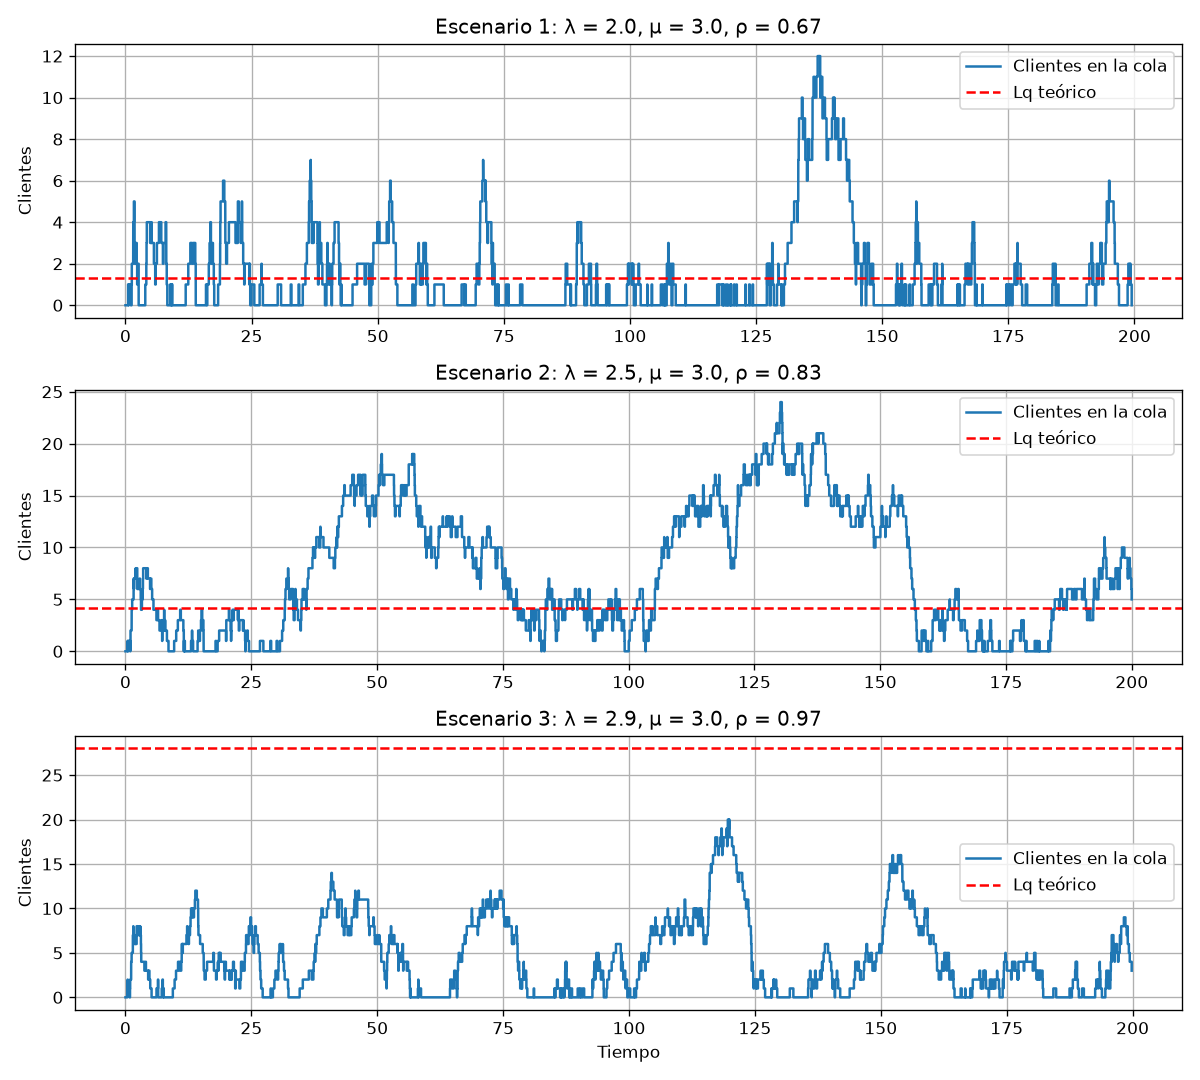
\includegraphics[width=\textwidth]{figures/cola_en_el_tiempo.png}
\caption{Clientes en la cola a lo largo del tiempo, un panel por escenario, con la línea
roja del valor teórico $L_q$. La escala vertical crece con $\lambda$: en el escenario 1
las oscilaciones son de pocos clientes y en el escenario 3 se registran ráfagas de hasta
20 clientes.}
\label{fig:cola}
\end{figure}

La Figura~\ref{fig:esperas} muestra el tiempo que esperó cada uno de los primeros 300
clientes, con la línea del valor teórico $W_q$.

\begin{figure}[h!]
\centering
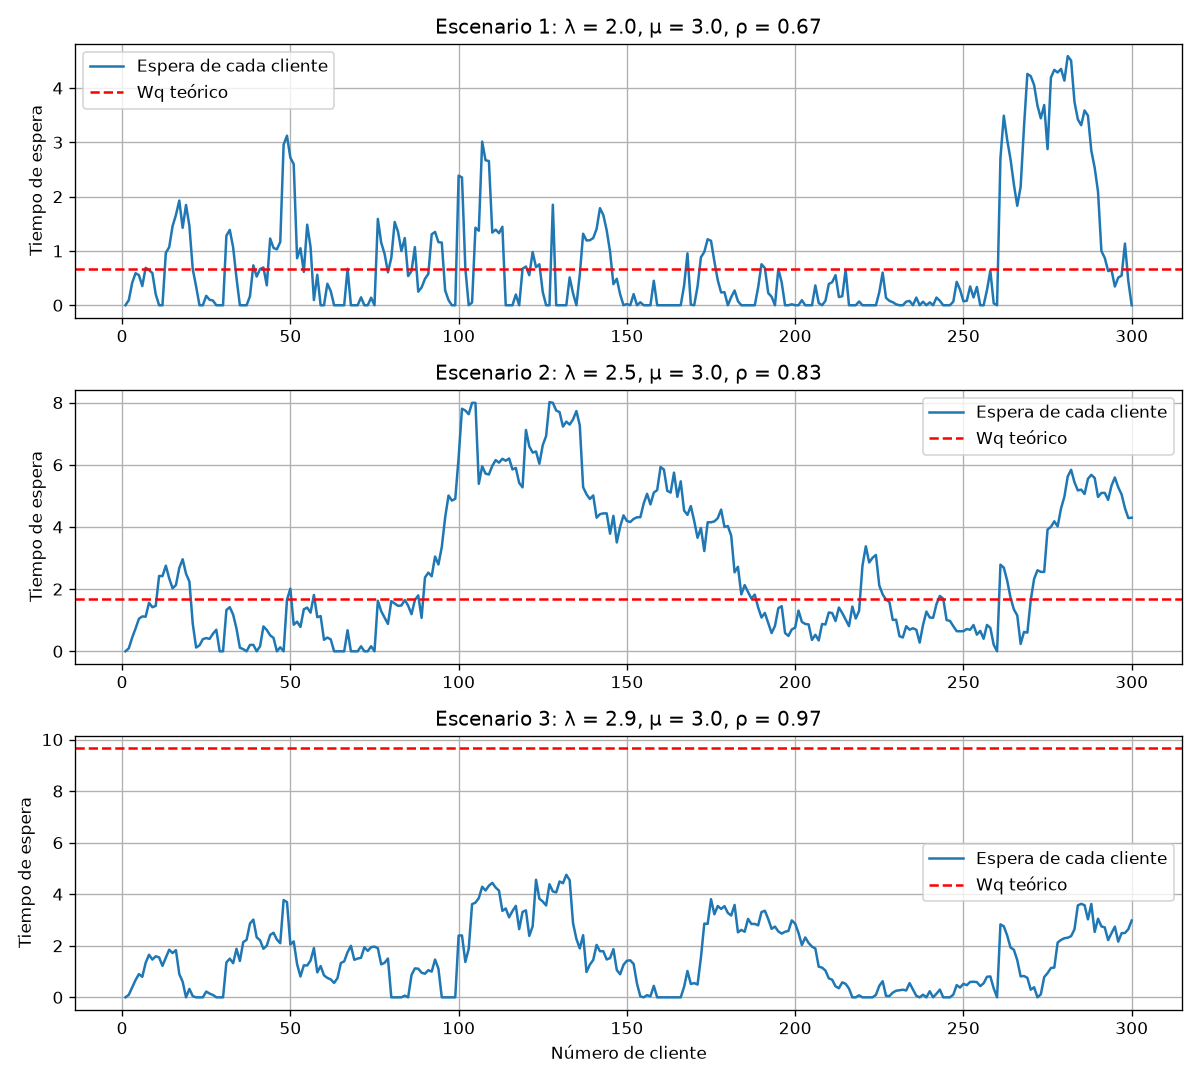
\includegraphics[width=\textwidth]{figures/tiempos_de_espera.png}
\caption{Tiempo de espera de cada cliente (primeros 300), un panel por escenario, con la
línea roja del valor teórico $W_q$. La dispersión de la serie crece con $\rho$: en el
escenario 1 las esperas son pequeñas y casi constantes, y en los escenarios 2 y 3
aparecen tramos largos muy por encima del valor teórico.}
\label{fig:esperas}
\end{figure}

La Figura~\ref{fig:comparacion} compara, con barras, el valor teórico y el valor
simulado de $W_q$ y de $L_q$ en los tres escenarios.

\begin{figure}[h!]
\centering
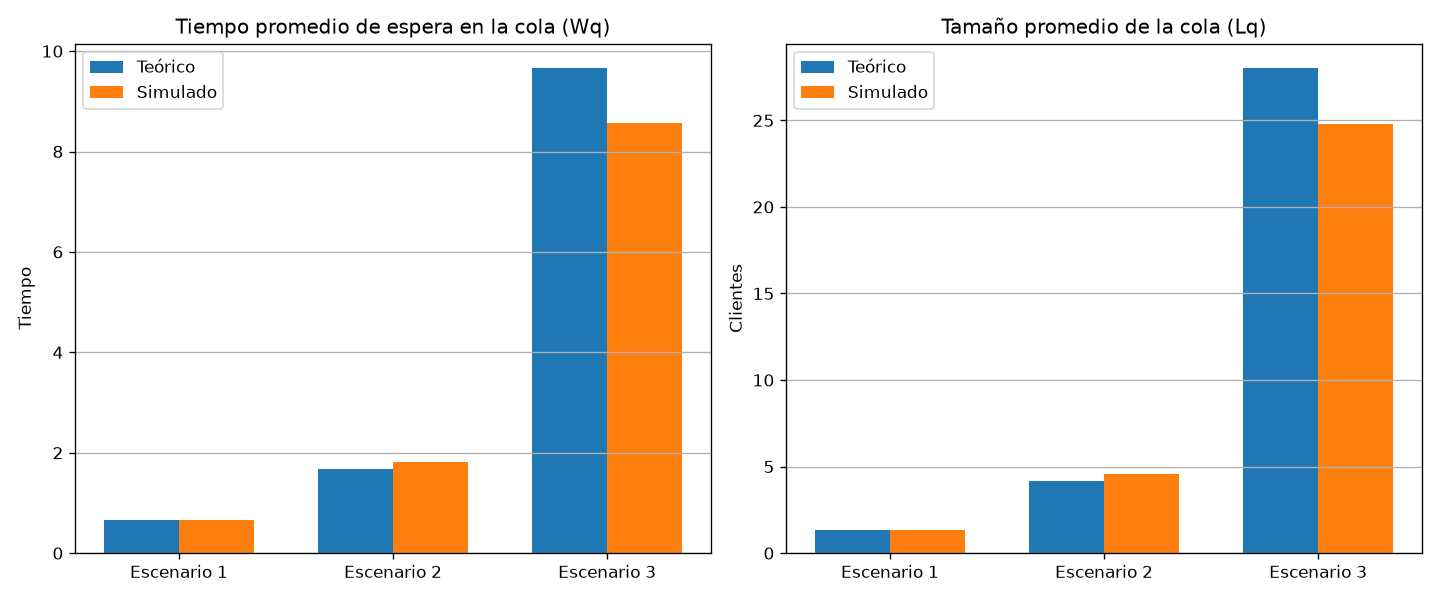
\includegraphics[width=\textwidth]{figures/teoria_vs_simulacion.png}
\caption{Comparación teoría -- simulación por escenario para $W_q$ (izquierda) y $L_q$
(derecha). Las barras azules son los valores teóricos y las naranjas el promedio de las
10 réplicas simuladas.}
\label{fig:comparacion}
\end{figure}

\section{Análisis de Resultados}

\pendiente{el análisis escrito de las gráficas y de la comparación teoría--simulación.
Debe cubrir: (a)~cómo crecen $W_q$ y $L_q$ al acercarse $\lambda$ a $\mu$ y por qué el
crecimiento es acelerado y no proporcional; (b)~por qué lo simulado no coincide
exactamente con lo teórico, distinguiendo el error de muestreo del sesgo de
implementación; (c)~qué significa que el valor teórico caiga dentro del intervalo de
confianza; (d)~por qué cerca de la saturación una corrida individual no es evidencia
suficiente.}

\section{Preguntas de Control}

\noindent\pendiente{respuestas del equipo a las 10 preguntas de la guía.}

\begin{enumerate}
    \item \textbf{\textquestiondown{}Qué representa el modelo M/M/1?}
    \par\vspace{1.5em}
    \item \textbf{\textquestiondown{}Qué representan $\lambda$ y $\mu$?}
    \par\vspace{1.5em}
    \item \textbf{\textquestiondown{}Por qué debe cumplirse $\lambda < \mu$ para que el
    sistema sea estable?}
    \par\vspace{1.5em}
    \item \textbf{\textquestiondown{}Qué significa la utilización $\rho$?}
    \par\vspace{1.5em}
    \item \textbf{\textquestiondown{}Cuál es la diferencia entre $W$ y $W_q$?}
    \par\vspace{1.5em}
    \item \textbf{\textquestiondown{}Cuál es la diferencia entre $L$ y $L_q$?}
    \par\vspace{1.5em}
    \item \textbf{\textquestiondown{}Por qué SimPy utiliza una distribución exponencial
    para generar los tiempos?}
    \par\vspace{1.5em}
    \item \textbf{\textquestiondown{}Qué sucede con la cola cuando $\lambda$ se aproxima
    a $\mu$?}
    \par\vspace{1.5em}
    \item \textbf{\textquestiondown{}Por qué los resultados simulados pueden ser
    diferentes de los resultados teóricos?}
    \par\vspace{1.5em}
    \item \textbf{\textquestiondown{}Qué ocurriría si $\lambda$ fuera mayor que $\mu$?}
    \par\vspace{1.5em}
\end{enumerate}

\section{Conclusiones}

\pendiente{las conclusiones, una por cada objetivo de la práctica y atadas a los
resultados de la Tabla~\ref{tab:comparacion} y la Tabla~\ref{tab:intervalos}.}

\section{Demostración}

El video de demostración debe mostrar la ejecución del programa desde la línea de
comandos: la corrida de los tres escenarios, las dos tablas que se imprimen en la
terminal y la generación de las tres gráficas en la carpeta \texttt{graficas/}.

\pendiente{enlace al video de demostración.}

\section{Bibliografía}

\nocite{*}
\bibliographystyle{plain}
\bibliography{referencias}

\end{document}
